% Copie LaTeX de README.md (projet Assurance de risque), générée par
% generation/generer_latex.py. Compilation : pdflatex, xelatex ou lualatex
% (deux passes pour la table des matières), depuis ce dossier.
% Options for packages loaded elsewhere

\PassOptionsToPackage{unicode}{hyperref}

\PassOptionsToPackage{hyphens}{url}

\PassOptionsToPackage{dvipsnames,svgnames,x11names}{xcolor}

\documentclass[

  french,

  10pt,

  a4paper,

]{article}

\usepackage{xcolor}

\usepackage[margin=2cm]{geometry}

\usepackage{amsmath,amssymb}

\setcounter{secnumdepth}{-\maxdimen} % remove section numbering

\usepackage{iftex}

\ifPDFTeX

  \usepackage[T1]{fontenc}

  \usepackage[utf8]{inputenc}

  \usepackage{textcomp} % provide euro and other symbols

\else % if luatex or xetex

  \usepackage{unicode-math} % this also loads fontspec

  \defaultfontfeatures{Scale=MatchLowercase}

  \defaultfontfeatures[\rmfamily]{Ligatures=TeX,Scale=1}

\fi

\usepackage{lmodern}

\ifPDFTeX\else

  % xetex/luatex font selection

\fi

% Use upquote if available, for straight quotes in verbatim environments

\IfFileExists{upquote.sty}{\usepackage{upquote}}{}

\IfFileExists{microtype.sty}{% use microtype if available

  \usepackage[]{microtype}

  \UseMicrotypeSet[protrusion]{basicmath} % disable protrusion for tt fonts

}{}

\makeatletter

\@ifundefined{KOMAClassName}{% if non-KOMA class

  \IfFileExists{parskip.sty}{%

    \usepackage{parskip}

  }{% else

    \setlength{\parindent}{0pt}

    \setlength{\parskip}{6pt plus 2pt minus 1pt}}

}{% if KOMA class

  \KOMAoptions{parskip=half}}

\makeatother

\usepackage{longtable,booktabs,array}

\newcounter{none} % for unnumbered tables

\usepackage{calc} % for calculating minipage widths

% Correct order of tables after \paragraph or \subparagraph

\usepackage{etoolbox}

\makeatletter

\patchcmd\longtable{\par}{\if@noskipsec\mbox{}\fi\par}{}{}

\makeatother

% Allow footnotes in longtable head/foot

\IfFileExists{footnotehyper.sty}{\usepackage{footnotehyper}}{\usepackage{footnote}}

\makesavenoteenv{longtable}

\usepackage{graphicx}

\makeatletter

\newsavebox\pandoc@box

\newcommand*\pandocbounded[1]{% scales image to fit in text height/width

  \sbox\pandoc@box{#1}%

  \Gscale@div\@tempa{\textheight}{\dimexpr\ht\pandoc@box+\dp\pandoc@box\relax}%

  \Gscale@div\@tempb{\linewidth}{\wd\pandoc@box}%

  \ifdim\@tempb\p@<\@tempa\p@\let\@tempa\@tempb\fi% select the smaller of both

  \ifdim\@tempa\p@<\p@\scalebox{\@tempa}{\usebox\pandoc@box}%

  \else\usebox{\pandoc@box}%

  \fi%

}

% Set default figure placement to htbp

\def\fps@figure{htbp}

\makeatother

\ifLuaTeX

\usepackage[bidi=basic,shorthands=off]{babel}

\else

\usepackage[bidi=default,shorthands=off]{babel}

\fi

\ifLuaTeX

  \usepackage{selnolig} % disable illegal ligatures

\fi

\setlength{\emergencystretch}{3em} % prevent overfull lines

\providecommand{\tightlist}{%

  \setlength{\itemsep}{0pt}\setlength{\parskip}{0pt}}

% En-tête ajouté au modèle LaTeX de Pandoc pour les copies des README du projet.

% N'utilise que des extensions standard (float, etoolbox), présentes dans TeX Live,

% MiKTeX et Overleaf.

\usepackage{float}

\floatplacement{figure}{H}               % chaque figure reste à sa place dans le texte

\usepackage{etoolbox}

\AtBeginEnvironment{longtable}{\small}   % tableaux en petit corps

\setlength{\tabcolsep}{4pt}

\makeatletter

\renewcommand{\verbatim@font}{\small\ttfamily}  % blocs de code (commandes, arborescence)

\makeatother

\usepackage{bookmark}

\IfFileExists{xurl.sty}{\usepackage{xurl}}{} % add URL line breaks if available

\urlstyle{same}

\hypersetup{

  pdftitle={Étape 1.0 --- Présentation des données},

  pdflang={fr},

  colorlinks=true,

  linkcolor={blue},

  filecolor={Maroon},

  citecolor={Blue},

  urlcolor={blue},

  pdfcreator={LaTeX via pandoc}}



\title{Étape 1.0 --- Présentation des données}

\author{}

\date{}



\begin{document}

\maketitle



{

\hypersetup{linkcolor=black}

\setcounter{tocdepth}{3}

\tableofcontents

}

\begin{quote}

\textbf{Énoncé (partie 1)} : présenter les variables disponibles et préciser leur nature ; identifier les variables cibles de la segmentation et des analyses de fréquence et de gravité ; réaliser une analyse descriptive ; présenter un tableau récapitulatif de la base.

\end{quote}



\section{Exécution}



\begin{verbatim}

.venv\Scripts\python.exe partie1_donnees\1.0_presentation\etape_1_0_presentation.py

\end{verbatim}



\textbf{Notebook} (déjà exécuté : tableaux et figures visibles sans rien relancer) : \href{etape_1_0_presentation.ipynb}{\texttt{etape\_1\_0\_presentation.ipynb}}. \textbf{Version LaTeX} de ce document : \texttt{README.tex}.



{\def\LTcaptype{none} % do not increment counter

\begin{longtable}[]{@{}

  >{\raggedright\arraybackslash}p{(\linewidth - 2\tabcolsep) * \real{0.5000}}

  >{\raggedright\arraybackslash}p{(\linewidth - 2\tabcolsep) * \real{0.5000}}@{}}

\toprule\noalign{}

\begin{minipage}[b]{\linewidth}\raggedright

Entrée

\end{minipage} & \begin{minipage}[b]{\linewidth}\raggedright

Sorties

\end{minipage} \\

\midrule\noalign{}

\endhead

\bottomrule\noalign{}

\endlastfoot

\texttt{sources/InsuranceData.xlsx} (feuille \texttt{DataUsed}) & \texttt{resultats/tables/*.csv}, \texttt{resultats/figures/*.png}, \texttt{resultats/journal.txt} \\

\end{longtable}

}



Les données ne sont pas modifiées à cette étape. On décrit le fichier \textbf{tel qu'il a été saisi}.



\begin{center}\rule{0.5\linewidth}{0.5pt}\end{center}



\section{1. Tableau récapitulatif de la base}



{\def\LTcaptype{none} % do not increment counter

\begin{longtable}[]{@{}ll@{}}

\toprule\noalign{}

Caractéristique & Valeur \\

\midrule\noalign{}

\endhead

\bottomrule\noalign{}

\endlastfoot

Observations (individus enquêtés) & \textbf{4 076} \\

Variables & \textbf{73} \\

dont identifiant & 1 (\texttt{id}) \\

dont quantitatives & 22 \\

dont qualitatives & 47 (30 nominales, 17 ordinales) \\

dont texte libre & 3 \\

Variables stockées en nombre dans Excel & 9 \\

Variables quantitatives \textbf{saisies en texte} & 14 \\

Cellules manquantes & 15,7 \% du total \\

Variables avec plus de 50 \% de manquants & 10 \\

Variables sans aucun manquant & 1 (\texttt{id}) \\

Lignes en double (hors identifiant) & 2 \\

Identifiant unique & oui \\

\end{longtable}

}



L'énoncé annonce 4 077 individus : l'écart d'une unité correspond à la ligne d'en-tête du fichier Excel.



\section{2. Les variables et leur nature}



Les intitulés d'origine, longs et bilingues (français / malgache), ont été remplacés par des \textbf{codes courts} (dictionnaire complet ci-dessous et dans \texttt{resultats/tables/dictionnaire\_variables.csv}).



{\def\LTcaptype{none} % do not increment counter

\begin{longtable}[]{@{}

  >{\raggedright\arraybackslash}p{(\linewidth - 4\tabcolsep) * \real{0.3333}}

  >{\raggedright\arraybackslash}p{(\linewidth - 4\tabcolsep) * \real{0.3333}}

  >{\raggedright\arraybackslash}p{(\linewidth - 4\tabcolsep) * \real{0.3333}}@{}}

\toprule\noalign{}

\begin{minipage}[b]{\linewidth}\raggedright

Bloc thématique

\end{minipage} & \begin{minipage}[b]{\linewidth}\raggedright

Nb

\end{minipage} & \begin{minipage}[b]{\linewidth}\raggedright

Variables

\end{minipage} \\

\midrule\noalign{}

\endhead

\bottomrule\noalign{}

\endlastfoot

Identifiant & 1 & id \\

Démographie & 6 & sexe, age, fokotany, lien\_chef\_menage, statut\_matrimonial, niveau\_etude \\

Activité professionnelle & 9 & statut\_pro, secteur, activite\_famille, anciennete\_emploi, distance\_travail, transport\_travail, heures\_jour, jours\_semaine, nb\_employes \\

Ménage et logement & 8 & taille\_menage, nb\_actifs\_menage, activite\_conjoint, statut\_residence, source\_eau, source\_electricite, energie\_cuisine, type\_toilette \\

Revenus et budget & 6 & revenu, budget\_alim, budget\_sante, budget\_elec, epargne, dettes \\

Conditions de travail & 6 & effort\_physique, duree\_effort, pb\_sante\_travail, arret\_maladie, impact\_travail\_sante, repos\_recent \\

Couverture maladie & 6 & couverture, mode\_affiliation, type\_couverture, ancienne\_couverture, interet\_couverture, prime\_souhaitee \\

État de santé & 12 & maladie\_chronique, chronique\_categorie, chronique\_detail, traitement\_regulier, freq\_consult\_chronique, depense\_medic\_chronique, lunettes, valeur\_lunettes, dentiste, freq\_dentiste, \textbf{nb\_maladies\_graves}, renoncement\_soins \\

Dernier épisode de maladie & 10 & date\_derniere\_maladie, type\_maladie, douleur, jours\_arret, type\_recours, motif\_recours, distance\_soins, satisfaction, autre\_recours\_souhaite, benefice\_autre\_recours \\

Coûts du dernier épisode & 6 & \textbf{cout\_consultation, cout\_hospitalisation, cout\_medicaments, cout\_deplacement, cout\_alimentation, cout\_autres} \\

Impact sur l'activité & 3 & impact\_autre, impact\_maladie\_activite, recuperation\_activite \\

\end{longtable}

}



\textbf{Nature des variables :}



\begin{itemize}

\tightlist

\item

  \textbf{Quantitatives continues} (17) : âge, parts de budget, prime souhaitée, six coûts, deux distances, ancienneté, heures de travail, durée d'arrêt, dépense en médicaments.

\item

  \textbf{Quantitatives discrètes} (5) : taille du ménage, nombre d'actifs, jours travaillés par semaine, nombre d'employés, \textbf{nombre de maladies graves}.

\item

  \textbf{Qualitatives nominales} (30) : sexe, statut, secteur, logement, recours aux soins, réponses oui / non\ldots{}

\item

  \textbf{Qualitatives ordinales} (17) : niveau d'étude, tranche de revenu, échelles de fréquence ou d'intensité (effort physique, problèmes de santé, douleur, satisfaction\ldots).

\item

  \textbf{Texte libre} (3) : date et type de la dernière maladie, détail des maladies chroniques.

\end{itemize}



\textbf{Dictionnaire complet des 73 variables}



{\def\LTcaptype{none} % do not increment counter

\begin{longtable}[]{@{}

  >{\raggedright\arraybackslash}p{(\linewidth - 12\tabcolsep) * \real{0.1429}}

  >{\raggedright\arraybackslash}p{(\linewidth - 12\tabcolsep) * \real{0.1429}}

  >{\raggedright\arraybackslash}p{(\linewidth - 12\tabcolsep) * \real{0.1429}}

  >{\raggedright\arraybackslash}p{(\linewidth - 12\tabcolsep) * \real{0.1429}}

  >{\raggedright\arraybackslash}p{(\linewidth - 12\tabcolsep) * \real{0.1429}}

  >{\raggedleft\arraybackslash}p{(\linewidth - 12\tabcolsep) * \real{0.1429}}

  >{\raggedleft\arraybackslash}p{(\linewidth - 12\tabcolsep) * \real{0.1429}}@{}}

\toprule\noalign{}

\begin{minipage}[b]{\linewidth}\raggedright

code

\end{minipage} & \begin{minipage}[b]{\linewidth}\raggedright

libellé d'origine (tronqué)

\end{minipage} & \begin{minipage}[b]{\linewidth}\raggedright

bloc

\end{minipage} & \begin{minipage}[b]{\linewidth}\raggedright

nature

\end{minipage} & \begin{minipage}[b]{\linewidth}\raggedright

stockage Excel

\end{minipage} & \begin{minipage}[b]{\linewidth}\raggedleft

valeurs distinctes

\end{minipage} & \begin{minipage}[b]{\linewidth}\raggedleft

\% manquants

\end{minipage} \\

\midrule\noalign{}

\endhead

\bottomrule\noalign{}

\endlastfoot

id & N & Identifiant & Identifiant & nombre & 4076 & 0.0 \\

sexe & Sexe & Démographie & Qualitative nominale & texte & 4 & 0.2 \\

age & Age & Démographie & Quantitative continue & nombre & 53 & 0.2 \\

fokotany & Fokotany & Démographie & Qualitative nominale & texte & 237 & 0.1 \\

lien\_chef\_menage & Statut familiale & Démographie & Qualitative nominale & texte & 8 & 0.5 \\

statut\_pro & statut du professionnel & Activité professionnelle & Qualitative nominale & texte & 6 & 0.2 \\

statut\_matrimonial & Statut personnel & Démographie & Qualitative nominale & texte & 5 & 0.3 \\

taille\_menage & Effectif du ménage & Ménage et logement & Quantitative discrète & nombre & 18 & 0.1 \\

nb\_actifs\_menage & Nombre de personne qui travaille & Ménage et logement & Quantitative discrète & nombre & 8 & 0.1 \\

secteur & Votre secteur d'activité & Activité professionnelle & Qualitative nominale & texte & 103 & 0.4 \\

activite\_conjoint & Activité du conjoint & Ménage et logement & Qualitative nominale & texte & 17 & 30.3 \\

niveau\_etude & Niveau d'étude & Démographie & Qualitative ordinale & texte & 8 & 0.2 \\

statut\_residence & Statut Résidence & Ménage et logement & Qualitative nominale & texte & 2 & 0.1 \\

source\_eau & Type fournisseur eau & Ménage et logement & Qualitative nominale & texte & 9 & 0.2 \\

source\_electricite & Type fournisseur Electricité & Ménage et logement & Qualitative nominale & texte & 21 & 0.2 \\

energie\_cuisine & Energie Cuisine & Ménage et logement & Qualitative nominale & texte & 15 & 0.2 \\

type\_toilette & Type de toilette & Ménage et logement & Qualitative nominale & texte & 5 & 0.3 \\

activite\_famille & Principal activité de la famille & Activité professionnelle & Qualitative nominale & texte & 59 & 55.2 \\

anciennete\_emploi & Ancienneté emploi & Activité professionnelle & Quantitative continue & texte (nombres saisis en texte) & 451 & 0.4 \\

distance\_travail & Distance travail & Activité professionnelle & Quantitative continue & texte (nombres saisis en texte) & 475 & 0.7 \\

transport\_travail & Transport travail & Activité professionnelle & Qualitative nominale & texte & 26 & 0.5 \\

heures\_jour & Heures travaillées quotidiennes & Activité professionnelle & Quantitative continue & texte (nombres saisis en texte) & 216 & 0.3 \\

jours\_semaine & Nombre de jours travaillés par semaine & Activité professionnelle & Quantitative discrète & texte (nombres saisis en texte) & 128 & 0.3 \\

nb\_employes & Votre Nombre employés & Activité professionnelle & Quantitative discrète & texte (nombres saisis en texte) & 95 & 16.6 \\

revenu & Votre Revenu mensuel & Revenus et budget & Qualitative ordinale & texte & 24 & 1.1 \\

budget\_alim & \% Budget alimentation & Revenus et budget & Quantitative continue & nombre & 97 & 2.8 \\

budget\_sante & \% Budget santé & Revenus et budget & Quantitative continue & nombre & 35 & 5.1 \\

budget\_elec & \% Budget électricité & Revenus et budget & Quantitative continue & nombre & 33 & 5.0 \\

epargne & Avoir de l'épargne & Revenus et budget & Qualitative nominale & texte & 2 & 0.2 \\

dettes & Avoir des Dettes impayées & Revenus et budget & Qualitative nominale & texte & 2 & 0.2 \\

effort\_physique & Effort physique au travail & Conditions de travail & Qualitative ordinale & texte & 6 & 0.4 \\

duree\_effort & Durée de l'effort & Conditions de travail & Qualitative ordinale & texte & 4 & 0.4 \\

pb\_sante\_travail & Problèmes de Santé au travail & Conditions de travail & Qualitative ordinale & texte & 7 & 0.3 \\

arret\_maladie & Arrêt maladie lieu au travail & Conditions de travail & Qualitative ordinale & texte & 5 & 0.3 \\

impact\_travail\_sante & Impact du travail sur votre santé & Conditions de travail & Qualitative ordinale & texte & 4 & 0.3 \\

repos\_recent & Repos travail récemment & Conditions de travail & Qualitative ordinale & texte & 3 & 0.3 \\

couverture & Affiliation Couverture maladie & Couverture maladie & Qualitative nominale & texte & 2 & 0.4 \\

mode\_affiliation & Mode affiliation & Couverture maladie & Qualitative nominale & texte & 7 & 97.5 \\

type\_couverture & Type couverture & Couverture maladie & Qualitative nominale & texte & 13 & 97.5 \\

ancienne\_couverture & Ancienne couverture & Couverture maladie & Qualitative nominale & texte & 2 & 3.0 \\

interet\_couverture & Avantage adhérer à une couverture & Couverture maladie & Qualitative ordinale & texte & 7 & 0.3 \\

prime\_souhaitee & Votre avis du Prime mensuelle & Couverture maladie & Quantitative continue & nombre & 51 & 3.4 \\

maladie\_chronique & Souffrez-vous de Maladies chroniques & État de santé & Qualitative nominale & texte & 3 & 0.3 \\

chronique\_categorie & Quelles, maladies chroniques & État de santé & Qualitative nominale & texte & 13 & 90.1 \\

chronique\_detail & type maladies chroniques & État de santé & Texte libre & texte & 171 & 92.1 \\

traitement\_regulier & Traitement médical régulier & État de santé & Qualitative ordinale & texte & 3 & 90.1 \\

freq\_consult\_chronique & Fréquence consultation cette maladie & État de santé & Qualitative ordinale & texte & 4 & 98.4 \\

depense\_medic\_chronique & Depense médicaments & État de santé & Quantitative continue & texte (nombres saisis en texte) & 30 & 98.7 \\

lunettes & Portez-vous des lunettes ? & État de santé & Qualitative nominale & texte & 2 & 0.3 \\

valeur\_lunettes & valeur approximative de vos lunettes & État de santé & Qualitative ordinale & texte & 4 & 93.9 \\

dentiste & Consultation d'un dentiste & État de santé & Qualitative ordinale & texte & 3 & 0.3 \\

freq\_dentiste & Frequence moyenne par an ? & État de santé & Qualitative ordinale & texte & 4 & 44.6 \\

nb\_maladies\_graves & Nombre de Maladies graves 12 mois & État de santé & Quantitative discrète & nombre & 28 & 0.7 \\

renoncement\_soins & Au cours des 12 derniers mois, avez-vous été malade sans consulter\ldots{} & État de santé & Qualitative nominale & texte & 4 & 1.9 \\

date\_derniere\_maladie & Quand avez-vous été dernièrement malade ? & Dernier épisode de maladie & Texte libre & texte & 590 & 2.2 \\

type\_maladie & Quel type de maladie avez-vous eue ? & Dernier épisode de maladie & Texte libre & texte & 859 & 2.8 \\

douleur & E.3. Degré de perception de la douleur & Dernier épisode de maladie & Qualitative ordinale & texte & 5 & 5.4 \\

jours\_arret & Durée totale de cessation d'activité (jours) & Dernier épisode de maladie & Quantitative continue & texte (nombres saisis en texte) & 280 & 4.1 \\

type\_recours & Type de recours & Dernier épisode de maladie & Qualitative nominale & texte & 47 & 5.4 \\

motif\_recours & F.3. Pourquoi avez-vous choisi ce type de recours ? & Dernier épisode de maladie & Qualitative nominale & texte & 259 & 5.8 \\

distance\_soins & Distance du lieu de consultation & Dernier épisode de maladie & Quantitative continue & texte (nombres saisis en texte) & 261 & 4.7 \\

satisfaction & F.4. Êtes-vous satisfait du traitement ? & Dernier épisode de maladie & Qualitative ordinale & texte & 5 & 5.7 \\

autre\_recours\_souhaite & F.5. Quelles autres dispositions auraient été plus appropriées ? & Dernier épisode de maladie & Qualitative nominale & texte & 42 & 88.7 \\

benefice\_autre\_recours & F.6. Ces dispositions auraient donné & Dernier épisode de maladie & Qualitative nominale & texte & 134 & 20.9 \\

cout\_consultation & G.1. Frais de consultation & Coûts du dernier épisode & Quantitative continue & texte (nombres saisis en texte) & 92 & 6.3 \\

cout\_hospitalisation & G.2. Frais d'hospitalisation & Coûts du dernier épisode & Quantitative continue & texte (nombres saisis en texte) & 51 & 7.3 \\

cout\_medicaments & G.3. Coûts des médicaments & Coûts du dernier épisode & Quantitative continue & texte (nombres saisis en texte) & 332 & 5.8 \\

cout\_deplacement & G.4. Coût lié au déplacement & Coûts du dernier épisode & Quantitative continue & texte (nombres saisis en texte) & 62 & 6.6 \\

cout\_alimentation & G.5. Alimentation supplémentaire & Coûts du dernier épisode & Quantitative continue & texte (nombres saisis en texte) & 109 & 7.2 \\

cout\_autres & G.6. Autres à préciser & Coûts du dernier épisode & Quantitative continue & texte (nombres saisis en texte) & 57 & 7.8 \\

impact\_autre & H.3. Autre impact de la maladie sur l'activité & Impact sur l'activité & Qualitative nominale & texte & 11 & 8.2 \\

impact\_maladie\_activite & H.4. Impact ressenti de la maladie sur l'activité & Impact sur l'activité & Qualitative ordinale & texte & 4 & 5.6 \\

recuperation\_activite & H.5. Récupération des activités perdues & Impact sur l'activité & Qualitative nominale & texte & 14 & 6.8 \\

\end{longtable}

}



\section{3. Variables cibles}



{\def\LTcaptype{none} % do not increment counter

\begin{longtable}[]{@{}

  >{\raggedright\arraybackslash}p{(\linewidth - 6\tabcolsep) * \real{0.2500}}

  >{\raggedright\arraybackslash}p{(\linewidth - 6\tabcolsep) * \real{0.2500}}

  >{\raggedright\arraybackslash}p{(\linewidth - 6\tabcolsep) * \real{0.2500}}

  >{\raggedright\arraybackslash}p{(\linewidth - 6\tabcolsep) * \real{0.2500}}@{}}

\toprule\noalign{}

\begin{minipage}[b]{\linewidth}\raggedright

Analyse

\end{minipage} & \begin{minipage}[b]{\linewidth}\raggedright

Variable cible

\end{minipage} & \begin{minipage}[b]{\linewidth}\raggedright

Rôle

\end{minipage} & \begin{minipage}[b]{\linewidth}\raggedright

Observations

\end{minipage} \\

\midrule\noalign{}

\endhead

\bottomrule\noalign{}

\endlastfoot

\textbf{Segmentation} (K-means, étape 2.1) & aucune : apprentissage non supervisé & Les assurés sont regroupés selon leur profil (démographie, situation socio-économique, conditions de travail, état de santé). Le \textbf{segment obtenu devient la variable cible de l'arbre CART} (étape 2.2). & 4 076 \\

\textbf{Fréquence} (GLM, étape 3.1) & \texttt{nb\_maladies\_graves} & \emph{N\_i} : nombre de maladies graves déclarées sur les 12 derniers mois (variable de comptage). & 4 047 renseignées \\

\textbf{Sévérité} (GLM, étape 3.2) & \texttt{cout\_total} = somme des six coûts G.1 à G.6 & \emph{S\_i} : coût (en Ariary) du dernier épisode de maladie, à la charge de l'assuré. Construit à l'étape 1.1 après conversion du texte libre. & 3 871 individus avec au moins un coût renseigné \\

\end{longtable}

}



Deux précisions de modélisation :



\begin{itemize}

\tightlist

\item

  \textbf{Exposition} : tous les individus sont observés sur la même période (12 mois). L'exposition vaut donc 1 pour tous et le modèle de fréquence n'a pas besoin de terme d'exposition (\emph{offset}).

\item

  \textbf{Sinistre} : un sinistre est une maladie grave. Le coût disponible est celui du \emph{dernier} épisode de maladie ; on l'utilise comme estimation du coût d'un sinistre. Le modèle de sévérité sera donc ajusté sur les individus ayant au moins un sinistre (\emph{N\_i} \ensuremath{\geq} 1) et un coût positif.

\end{itemize}



\section{4. Analyse descriptive des données brutes}



\subsection{4.1 Variables quantitatives stockées en nombre}



{\def\LTcaptype{none} % do not increment counter

\begin{longtable}[]{@{}

  >{\raggedright\arraybackslash}p{(\linewidth - 20\tabcolsep) * \real{0.0909}}

  >{\raggedleft\arraybackslash}p{(\linewidth - 20\tabcolsep) * \real{0.0909}}

  >{\raggedleft\arraybackslash}p{(\linewidth - 20\tabcolsep) * \real{0.0909}}

  >{\raggedleft\arraybackslash}p{(\linewidth - 20\tabcolsep) * \real{0.0909}}

  >{\raggedleft\arraybackslash}p{(\linewidth - 20\tabcolsep) * \real{0.0909}}

  >{\raggedleft\arraybackslash}p{(\linewidth - 20\tabcolsep) * \real{0.0909}}

  >{\raggedleft\arraybackslash}p{(\linewidth - 20\tabcolsep) * \real{0.0909}}

  >{\raggedleft\arraybackslash}p{(\linewidth - 20\tabcolsep) * \real{0.0909}}

  >{\raggedleft\arraybackslash}p{(\linewidth - 20\tabcolsep) * \real{0.0909}}

  >{\raggedleft\arraybackslash}p{(\linewidth - 20\tabcolsep) * \real{0.0909}}

  >{\raggedleft\arraybackslash}p{(\linewidth - 20\tabcolsep) * \real{0.0909}}@{}}

\toprule\noalign{}

\begin{minipage}[b]{\linewidth}\raggedright

Variable

\end{minipage} & \begin{minipage}[b]{\linewidth}\raggedleft

n

\end{minipage} & \begin{minipage}[b]{\linewidth}\raggedleft

Moyenne

\end{minipage} & \begin{minipage}[b]{\linewidth}\raggedleft

Écart-type

\end{minipage} & \begin{minipage}[b]{\linewidth}\raggedleft

Min

\end{minipage} & \begin{minipage}[b]{\linewidth}\raggedleft

Q1

\end{minipage} & \begin{minipage}[b]{\linewidth}\raggedleft

Médiane

\end{minipage} & \begin{minipage}[b]{\linewidth}\raggedleft

Q3

\end{minipage} & \begin{minipage}[b]{\linewidth}\raggedleft

P99

\end{minipage} & \begin{minipage}[b]{\linewidth}\raggedleft

Max

\end{minipage} & \begin{minipage}[b]{\linewidth}\raggedleft

Asymétrie

\end{minipage} \\

\midrule\noalign{}

\endhead

\bottomrule\noalign{}

\endlastfoot

age & 4 066 & 37,8 & 11,5 & \textbf{3} & 28 & 37 & 46 & 59 & \textbf{112} & 0,3 \\

taille\_menage & 4 071 & 4,5 & 1,9 & \textbf{\ensuremath{-}6} & 3 & 4 & 5 & 10 & \textbf{30} & 2,8 \\

nb\_actifs\_menage & 4 070 & 1,9 & 0,9 & 0 & 1 & 2 & 2 & 5 & 7 & 0,9 \\

budget\_alim (\%) & 3 963 & 264,1 & 5 670 & 0 & 45 & 50 & 70 & 100 & \textbf{250 000} & 35,2 \\

budget\_sante (\%) & 3 870 & 71,1 & 1 559 & 0 & 0 & 10 & 10 & 31,5 & \textbf{70 000} & 34,3 \\

budget\_elec (\%) & 3 873 & 27,2 & 481 & 0 & 1 & 5 & 10 & 25 & \textbf{17 000} & 27,0 \\

prime\_souhaitee (Ar) & 3 938 & 8 310 & 8 893 & \textbf{\ensuremath{-}5 000} & 2 000 & 5 000 & 10 000 & 30 000 & 200 000 & 4,2 \\

nb\_maladies\_graves & 4 047 & 2,25 & 13,8 & \textbf{\ensuremath{-}1} & 1 & 1 & 2 & 10 & \textbf{365} & 24,2 \\

\end{longtable}

}



Les quartiles sont cohérents, mais les extrêmes (en gras) révèlent des \textbf{erreurs de saisie} : âge de 3 ou 112 ans, ménage de \ensuremath{-}6 personnes, parts de budget supérieures à 100 \% (des montants en Ariary saisis à la place d'un pourcentage), 365 maladies graves par an. Les moyennes et écarts-types bruts ne sont donc pas interprétables : elles seront traitées aux étapes 1.1 (valeurs impossibles) et 1.2 (valeurs aberrantes).



\begin{figure}

\centering

\pandocbounded{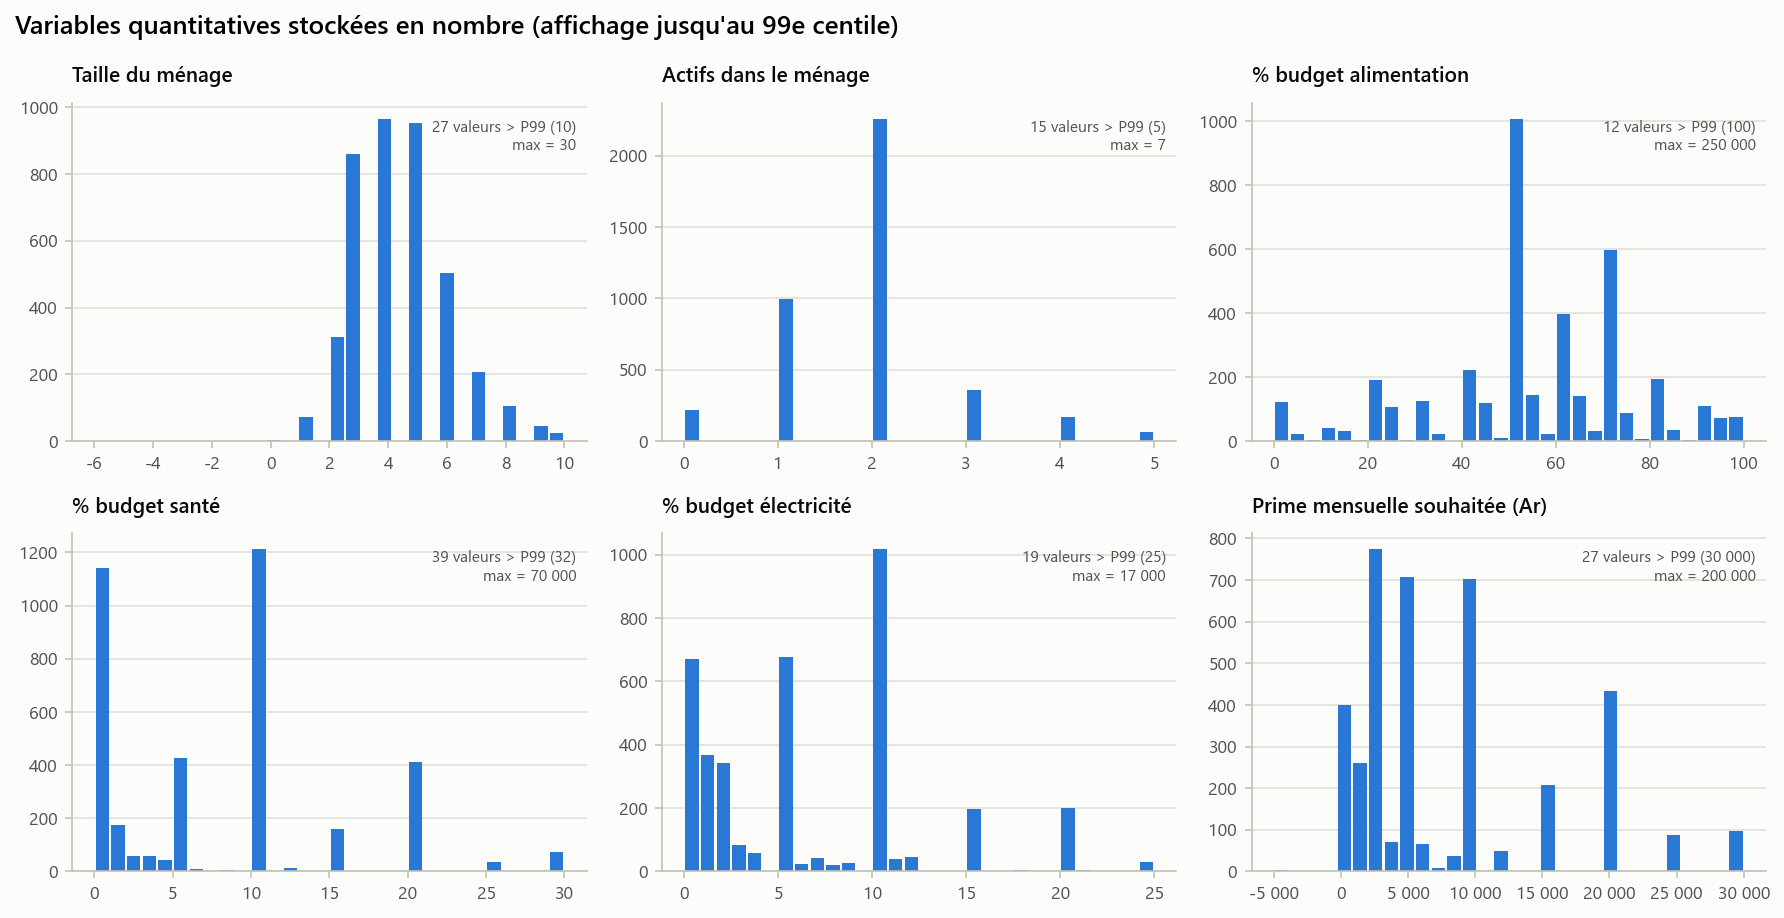
\includegraphics[keepaspectratio,alt={Variables quantitatives}]{resultats/figures/variables_quantitatives.png}}

\caption{Variables quantitatives}

\end{figure}



\subsection{4.2 Variables quantitatives saisies en texte}



14 variables numériques ont été saisies en texte libre. Elles mélangent nombres, unités et phrases en malgache.



{\def\LTcaptype{none} % do not increment counter

\begin{longtable}[]{@{}

  >{\raggedright\arraybackslash}p{(\linewidth - 6\tabcolsep) * \real{0.2500}}

  >{\raggedleft\arraybackslash}p{(\linewidth - 6\tabcolsep) * \real{0.2500}}

  >{\raggedleft\arraybackslash}p{(\linewidth - 6\tabcolsep) * \real{0.2500}}

  >{\raggedright\arraybackslash}p{(\linewidth - 6\tabcolsep) * \real{0.2500}}@{}}

\toprule\noalign{}

\begin{minipage}[b]{\linewidth}\raggedright

Variable

\end{minipage} & \begin{minipage}[b]{\linewidth}\raggedleft

Renseignées

\end{minipage} & \begin{minipage}[b]{\linewidth}\raggedleft

Nombres « purs »

\end{minipage} & \begin{minipage}[b]{\linewidth}\raggedright

Exemples de saisies non numériques

\end{minipage} \\

\midrule\noalign{}

\endhead

\bottomrule\noalign{}

\endlastfoot

anciennete\_emploi & 4 061 & 73,5 \% & \texttt{2ans}, \texttt{5ans}, \texttt{4taona} (taona = an) \\

distance\_travail & 4 046 & 53,8 \% & \texttt{1km}, \texttt{O}, \texttt{200m}, \texttt{Miovaova} (variable) \\

heures\_jour & 4 065 & 81,3 \% & \texttt{8h}, \texttt{Arakaraka} (ça dépend), \texttt{4\ \textasciitilde{}\ 5} \\

jours\_semaine & 4 064 & 80,9 \% & \texttt{6j}, \texttt{6/7}, \texttt{7/7} \\

nb\_employes & 3 401 & 79,9 \% & \texttt{O}, \texttt{Tsy\ mampiasa} (n'emploie personne) \\

jours\_arret & 3 907 & 72,8 \% & \texttt{Herinandro} (une semaine), \texttt{Niasa\ hiany} (a continué à travailler) \\

distance\_soins & 3 884 & 66,9 \% & \texttt{O}, \texttt{1km}, \texttt{9000\ mètre} \\

cout\_consultation \ldots{} cout\_autres & \ensuremath{\approx} 3 800 chacune & 82 à 94 \% & \texttt{O} (zéro), \texttt{Tsy\ nisy} (rien), \texttt{20\ 000}, \texttt{8000\ensuremath{\times}2:16000}, \texttt{Tambavy} (tisane) \\

\end{longtable}

}



Leur conversion en nombres est réalisée à l'étape 1.1.



\subsection{4.3 Variables qualitatives}



\begin{figure}

\centering

\pandocbounded{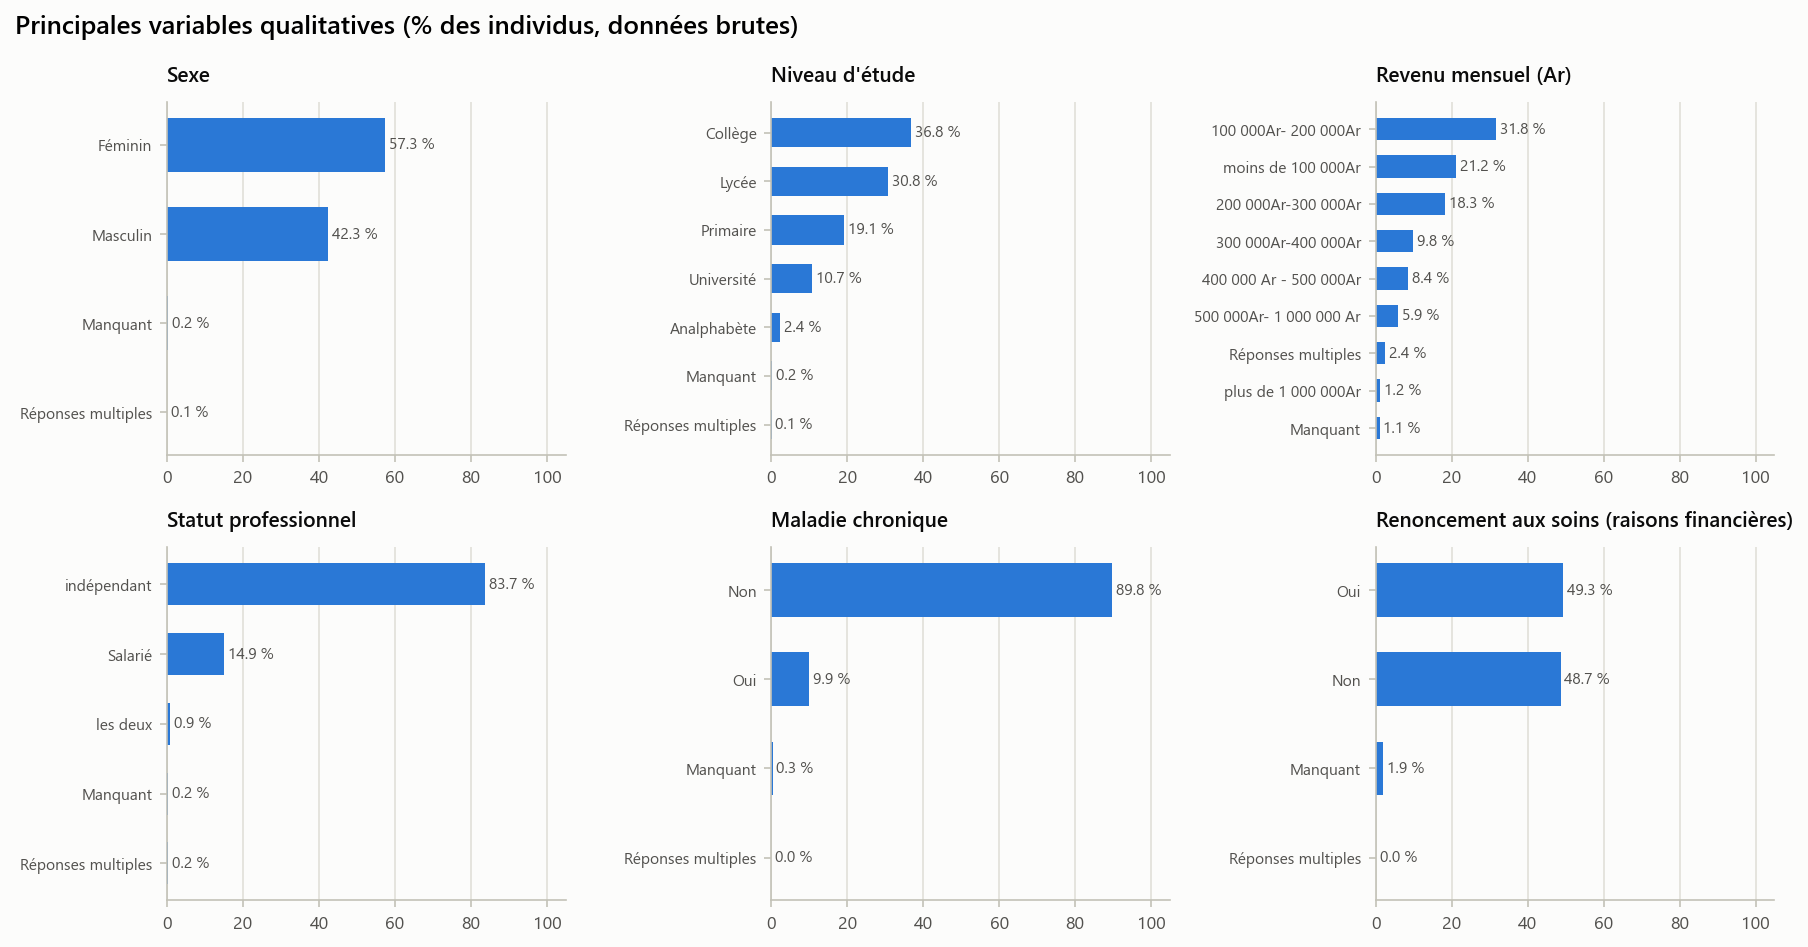
\includegraphics[keepaspectratio,alt={Principales variables qualitatives}]{resultats/figures/variables_qualitatives_principales.png}}

\caption{Principales variables qualitatives}

\end{figure}



\begin{itemize}

\tightlist

\item

  \textbf{Profil} : 57 \% de femmes ; 53 \% de chefs de ménage ; 70 \% de personnes mariées ; un niveau d'étude surtout collège (37 \%) et lycée (31 \%).

\item

  \textbf{Activité} : 84 \% d'indépendants, principalement dans l'agriculture et le commerce ; 80 \% se rendent au travail à pied.

\item

  \textbf{Revenus} : 53 \% gagnent moins de 200 000 Ar par mois ; seuls 26 \% ont une épargne et 14 \% ont des dettes impayées.

\item

  \textbf{Conditions de travail} : 52 \% font « toujours » un effort physique ; 43 \% ont « parfois » et 37 \% « régulièrement » des problèmes de santé au travail.

\item

  \textbf{Couverture maladie} : 97 \% \textbf{ne sont pas couverts}. C'est une variable quasi constante, donc peu exploitable pour la modélisation.

\item

  \textbf{Santé} : 10 \% ont une maladie chronique ; \textbf{49 \% ont renoncé à des soins pour raisons financières} au cours des 12 derniers mois.

\end{itemize}



\textbf{Réponses multiples} : plusieurs modalités sont parfois concaténées dans une même cellule (par exemple « Masculin Féminin », ou deux tranches de revenu). Le cas est rare pour les variables socio-démographiques (1 à 97 cellules), plus fréquent pour le secteur (355), l'électricité (193) et l'énergie de cuisine (190). Il est systématique pour les questions à choix multiples (\texttt{motif\_recours} : 1 588). Le détail figure dans \texttt{resume\_qualitatives.csv}.



\subsection{4.4 Variable de fréquence}



{\def\LTcaptype{none} % do not increment counter

\begin{longtable}[]{@{}

  >{\raggedright\arraybackslash}p{(\linewidth - 22\tabcolsep) * \real{0.0833}}

  >{\raggedleft\arraybackslash}p{(\linewidth - 22\tabcolsep) * \real{0.0833}}

  >{\raggedleft\arraybackslash}p{(\linewidth - 22\tabcolsep) * \real{0.0833}}

  >{\raggedleft\arraybackslash}p{(\linewidth - 22\tabcolsep) * \real{0.0833}}

  >{\raggedleft\arraybackslash}p{(\linewidth - 22\tabcolsep) * \real{0.0833}}

  >{\raggedleft\arraybackslash}p{(\linewidth - 22\tabcolsep) * \real{0.0833}}

  >{\raggedleft\arraybackslash}p{(\linewidth - 22\tabcolsep) * \real{0.0833}}

  >{\raggedleft\arraybackslash}p{(\linewidth - 22\tabcolsep) * \real{0.0833}}

  >{\raggedleft\arraybackslash}p{(\linewidth - 22\tabcolsep) * \real{0.0833}}

  >{\raggedleft\arraybackslash}p{(\linewidth - 22\tabcolsep) * \real{0.0833}}

  >{\raggedleft\arraybackslash}p{(\linewidth - 22\tabcolsep) * \real{0.0833}}

  >{\raggedleft\arraybackslash}p{(\linewidth - 22\tabcolsep) * \real{0.0833}}@{}}

\toprule\noalign{}

\begin{minipage}[b]{\linewidth}\raggedright

Sinistres

\end{minipage} & \begin{minipage}[b]{\linewidth}\raggedleft

0

\end{minipage} & \begin{minipage}[b]{\linewidth}\raggedleft

1

\end{minipage} & \begin{minipage}[b]{\linewidth}\raggedleft

2

\end{minipage} & \begin{minipage}[b]{\linewidth}\raggedleft

3

\end{minipage} & \begin{minipage}[b]{\linewidth}\raggedleft

4

\end{minipage} & \begin{minipage}[b]{\linewidth}\raggedleft

5

\end{minipage} & \begin{minipage}[b]{\linewidth}\raggedleft

6

\end{minipage} & \begin{minipage}[b]{\linewidth}\raggedleft

7--10

\end{minipage} & \begin{minipage}[b]{\linewidth}\raggedleft

\textgreater{} 10

\end{minipage} & \begin{minipage}[b]{\linewidth}\raggedleft

négatif

\end{minipage} & \begin{minipage}[b]{\linewidth}\raggedleft

manquant

\end{minipage} \\

\midrule\noalign{}

\endhead

\bottomrule\noalign{}

\endlastfoot

Individus & 943 & 1 311 & 1 030 & 399 & 177 & 103 & 24 & 20 & 39 & 1 & 29 \\

\end{longtable}

}



\begin{figure}

\centering

\pandocbounded{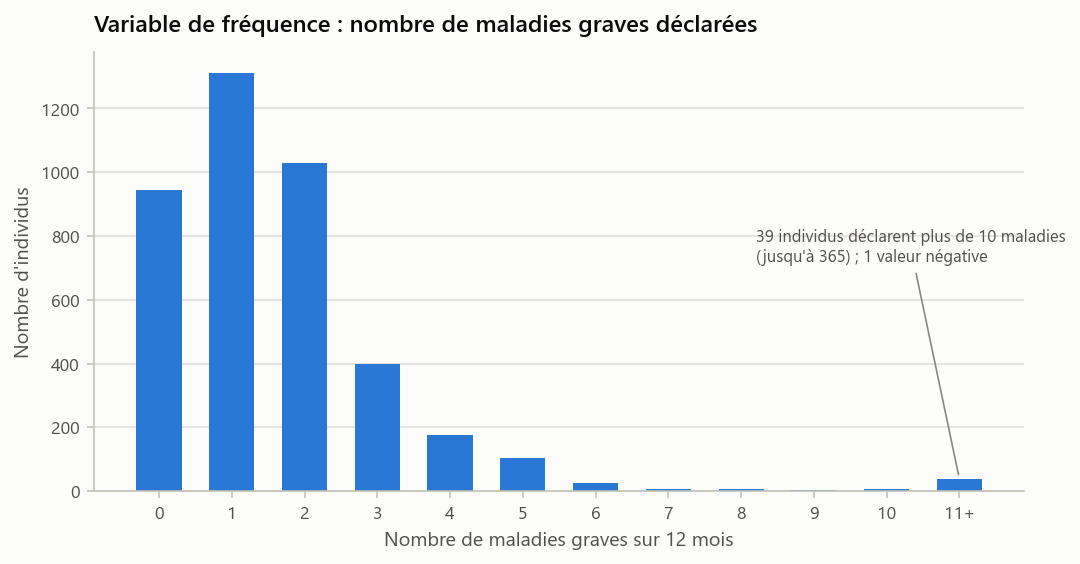
\includegraphics[keepaspectratio,alt={Distribution du nombre de maladies graves}]{resultats/figures/distribution_nb_maladies_graves.png}}

\caption{Distribution du nombre de maladies graves}

\end{figure}



La distribution a la forme attendue d'une variable de comptage (mode à 1, décroissance rapide). Le rapport variance / moyenne brut vaut \textbf{84,5}, mais il est dû à une quarantaine de valeurs extrêmes (jusqu'à 365) : la surdispersion sera réévaluée après traitement des valeurs aberrantes (étape 1.2), puis testée à l'étape 3.1 (choix entre Poisson et binomiale négative).



\subsection{4.5 Valeurs manquantes}



\begin{figure}

\centering

\pandocbounded{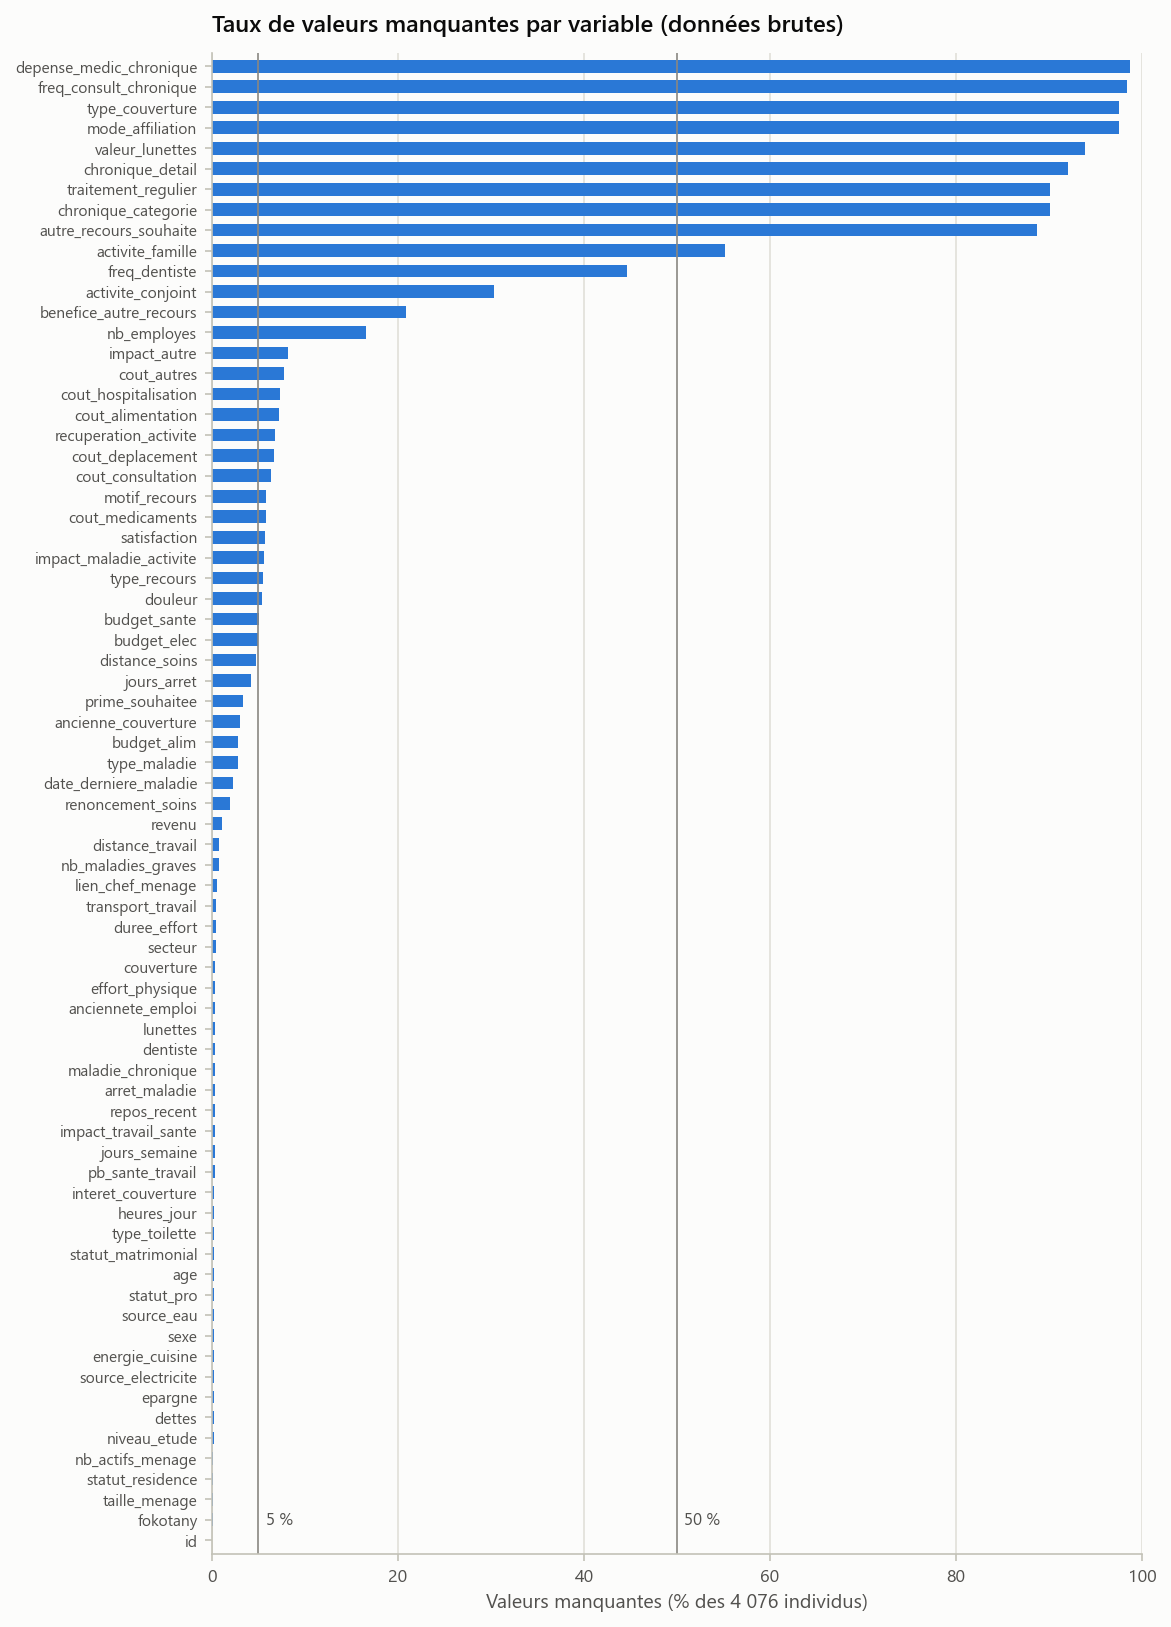
\includegraphics[keepaspectratio,alt={Taux de manquants par variable}]{resultats/figures/manquants_par_variable.png}}

\caption{Taux de manquants par variable}

\end{figure}



Trois groupes se dégagent :



\begin{enumerate}

\def\labelenumi{\arabic{enumi}.}

\tightlist

\item

  \textbf{Plus de 85 \% de manquants (9 variables)} : les questions conditionnelles posées seulement à une petite partie des répondants (détail des maladies chroniques, type de couverture, valeur des lunettes, F.5\ldots).

\item

  \textbf{Entre 15 et 55 \%} : \texttt{activite\_famille} (55 \%), \texttt{freq\_dentiste} (45 \%), \texttt{activite\_conjoint} (30 \%), \texttt{benefice\_autre\_recours} (21 \%), \texttt{nb\_employes} (17 \%).

\item

  \textbf{Moins de 10 \%} : toutes les autres variables. Les coûts et le bloc « dernier épisode de maladie » ont 4 à 8 \% de manquants, surtout chez les personnes qui n'ont pas été malades.

\end{enumerate}



\section{5. Constats pour l'étape suivante}



\begin{enumerate}

\def\labelenumi{\arabic{enumi}.}

\tightlist

\item

  \textbf{Identifiant} : \texttt{id} est unique et séquentiel ; il sert de clé mais ne sera jamais une variable explicative.

\item

  \textbf{Typage} : 14 variables numériques doivent être converties depuis le texte libre (français / malgache).

\item

  \textbf{Réponses multiples} : à résoudre pour une vingtaine de variables qualitatives.

\item

  \textbf{Valeurs impossibles} (âge, ménage, budgets, prime, fréquence négative) et \textbf{valeurs extrêmes} (fréquence jusqu'à 365, coûts) : à traiter aux étapes 1.1 et 1.2.

\item

  \textbf{Variables quasi vides ou quasi constantes} : à exclure en justifiant chaque décision.

\end{enumerate}



\ensuremath{\rightarrow} Suite : \href{../1.1_qualite/README.pdf}{étape 1.1 --- Qualité des données}



\section{Fichiers produits}



{\def\LTcaptype{none} % do not increment counter

\begin{longtable}[]{@{}

  >{\raggedright\arraybackslash}p{(\linewidth - 2\tabcolsep) * \real{0.5000}}

  >{\raggedright\arraybackslash}p{(\linewidth - 2\tabcolsep) * \real{0.5000}}@{}}

\toprule\noalign{}

\begin{minipage}[b]{\linewidth}\raggedright

Fichier

\end{minipage} & \begin{minipage}[b]{\linewidth}\raggedright

Contenu

\end{minipage} \\

\midrule\noalign{}

\endhead

\bottomrule\noalign{}

\endlastfoot

\texttt{resultats/tables/dictionnaire\_variables.csv} & 73 variables : code, intitulé d'origine, bloc, nature, stockage, modalités, \% manquants, exemples \\

\texttt{resultats/tables/tableau\_recapitulatif.csv} & Tableau récapitulatif de la base \\

\texttt{resultats/tables/variables\_cibles.csv} & Variables cibles et rôle \\

\texttt{resultats/tables/variables\_par\_nature.csv}, \texttt{variables\_par\_bloc.csv} & Répartition des variables \\

\texttt{resultats/tables/stats\_quantitatives.csv} & Statistiques descriptives des variables numériques \\

\texttt{resultats/tables/quantitatives\_saisies\_en\_texte.csv} & Variables numériques saisies en texte \\

\texttt{resultats/tables/frequences\_qualitatives.csv} & Effectifs de toutes les modalités brutes \\

\texttt{resultats/tables/resume\_qualitatives.csv} & Synthèse par variable qualitative (modalités, réponses multiples, modalité principale) \\

\texttt{resultats/tables/distribution\_nb\_maladies\_graves.csv} & Distribution de la variable de fréquence \\

\texttt{resultats/figures/*.png} & 5 figures \\

\texttt{resultats/journal.txt} & Sortie complète du script \\

\end{longtable}

}



\end{document}

